\subsection{Diseño de módulos de hardware del robot para pruebas de integración}
    %Parrafo 1
    En esta sección se detalla el diseño de los módulos de hardware del robot que hemos
        desarrollado para el Trabajo Terminal. El objetivo principal es asegurar una integración
        eficiente entre los diferentes componentes, permitiendo así la realización de pruebas
        de integración efectivas. La modularidad del diseño facilita tanto el desarrollo como el
        mantenimiento del sistema, así como también la sustitución de algunos componentes,
        esto nos permite aislar y solucionar problemas de manera aislada.
    \vskip 0.5cm
    %Parrafo 2
    Nuestro robot desarrollado consta de cuatro módulos principales: actuadores,
        sensores, unidad de control y módulo de visualización. Cada uno de estos módulos
        cumple una función especifica que permite al robot moverse, detectar obstáculos, y
        seguir rutas predefinidas.
    \vskip 0.5cm
    %Figura 1
    \begin{figure}[htbp]
        \centering
        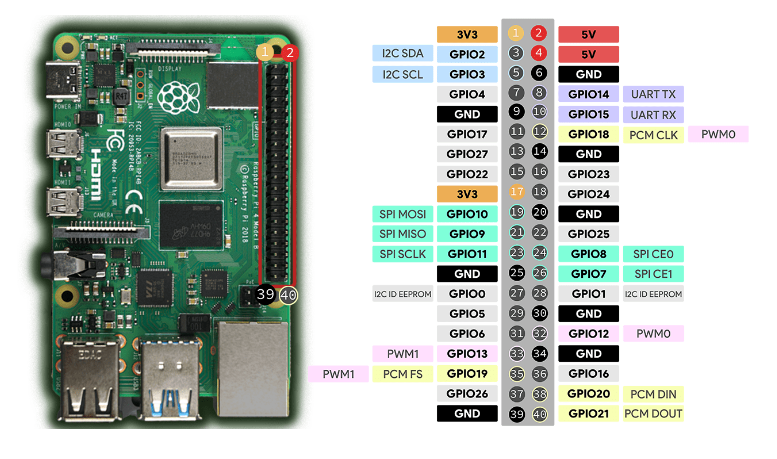
\includegraphics[width=0.5\textwidth]{./images/Pruebas/robot/robot01.png}
        \caption{Diseño de los pines de configuracion de los módulos de hardware del robot.}
        \label{fig:robot}
    \end{figure}

    \subsubsection{M\'odulo de actuadores (Motores)} % (fold)
    \label{ssub:modact}
    El robot está equipado por cuatro motores a pasos Nema 23, controlados a través de
        un controlador driver específico para motores a pasos. Estos motores son
        responsables del movimiento del robot en las direcciones deseadas, permitiendo giros,
        avances y retrocesos mediante la manipulación precisa de los pines de control PWM y
        de dirección.
    \vskip 0.5cm
    Los motores Nema 23 fueron elegidos debido a su precisión en el posicionamiento y
        su capacidad para generar el torque necesario para mover la estructura del robot, que
        está construida con perfiles de aluminio y ruedas omnidireccionales.
    \vskip 0.5cm
    % tabla 1
    \begin{longtable}{|c|c|c|c|}
        \hline
        \rowcolor{gray}
        \textbf{Producto} & \textbf{Descripci\'on} & \textbf{Piezas} \\
        \hline
        Motor a pasos Nema 23 & Motor a pasos Nema 23 con placa frontal & 4  \\
        Controlador de motores a pasos & Controlador de motores a pasos TB6600 & 4  \\
        Rueda omnidireccional & Rueda omnidireccional de 6 in & 4  \\
        \hline
        \caption{Especificaciones de los motores a pasos Nema 23.}
        \label{tab:motor}
    \end{longtable}
    \vskip 0.5cm
    Los motores están conectados a los pines GPIO de la Raspberry Pi 4 B mediante un
        controlador de moteres. El sistema de control utiliza señales PWM para regular la
        velocidad de los motores, y señales de dirección para controlar el sentido de giro.
    \vskip 0.5cm
    Elegimos los Motores Nema 23 debido a su precisión y capacidad de generar torque
        necesario para mover el robot con su estructura de aluminio y ruedas
        omnidireccionales. Su tamaño y especificaciones son ideales para aplicaciones que
        requieren alta precisión en el movimiento.
    \vskip 0.5cm
    La incorporación de ruedas omnidireccionales de 6 pulgadas permite al robot realizar
        movimientos en varias direcciones sin necesidad de girar su estructura por completo.
        Esto optimiza la maniobrabilidad en entornos reducidos
    \vskip 0.5cm
    Finalmente elegimos los controladores a pasos por que estos son capaces de manejar
        la corriente y el voltaje necesario para los motores Nema 23, permitiendo un control
        preciso mediante señales PWM generadas desde la unidad de control.}
    \vskip 0.5cm
    % subsubsection  (end)
    \subsubsection{M\'odulo de sensores} % (fold)
    \label{ssub:modsen}
    El robot está equipado por un sensor YLiDAR 2XL, que permite realizar un escaneo de
    360° del entorno para detectar obstáculos y mapear el área de operación del robot. La
    elección de este sensor se debe a su capacidad para medir distancias con alta
    precisión y su adecuado rango de operación, lo que lo convierte en una opción ideal
    para la navegación autónoma en tiempo real.
    El sensor se conecta a la unidad de control mediante un puerto USB tipo A.
    % subsubsection  (end)